% 共角共边相似（交叉对应）：△ABC 中 D∈AB、E∈AC，连 DE
% 当 AD/AC = AE/AB（即交叉相等）时，△ADE ∼ △ACB（注意对应顺序！）
\documentclass[tikz,border=4pt]{standalone}
\usetikzlibrary{calc}
\begin{document}
\begin{tikzpicture}[scale=1.0, thick]
  \coordinate (A) at (1, 4);
  \coordinate (B) at (-2.5, 0);
  \coordinate (C) at (3.5, 0);
  % 让 D 靠近 A（短边）、E 靠近 C（远）—— DE 与 BC "斜交"
  \coordinate (D) at ($(A)!0.35!(B)$);
  \coordinate (E) at ($(A)!0.75!(C)$);

  \draw (A) -- (B);
  \draw (A) -- (C);
  \draw (B) -- (C);
  \draw[blue, thick] (D) -- (E);

  % 长度标
  \node[above left]  at ($(A)!0.5!(D)$) {$AD$};
  \node[below left]  at ($(D)!0.5!(B)$) {};
  \node[above right] at ($(A)!0.5!(E)$) {$AE$};
  \node[below right] at ($(E)!0.5!(C)$) {};

  \node[above]       at (A) {$A$};
  \node[below left]  at (B) {$B$};
  \node[below right] at (C) {$C$};
  \node[left]        at (D) {$D$};
  \node[right]       at (E) {$E$};

  % 公共角 ∠A 标记（AB 方向 ≈ -131°，AC 方向 ≈ -58°）
  \draw ($(A) + ({0.55*cos(-131)}, {0.55*sin(-131)})$)
        arc[start angle=-131, end angle=-58, radius=0.55];
  \node at ($(A) + (0, -0.75)$) {\footnotesize $\angle A$};

  % 提示文字
  \node[align=left, font=\footnotesize] at (4.2, 3) {$\dfrac{AD}{AC}=\dfrac{AE}{AB}$\\\;\;$\Rightarrow \triangle ADE\sim\triangle ACB$};
\end{tikzpicture}
\end{document}
